\documentclass[11pt]{article}

\usepackage[utf8]{inputenc}
\usepackage[margin=1in]{geometry}
\usepackage{titlesec}
\usepackage[font={small, singlespacing},labelfont=bf]{caption}
\usepackage[doublespacing]{setspace}
\usepackage{listings}
\usepackage{hyperref}
\usepackage{lineno}
\linenumbers

\setlength{\parskip}{1em}

\usepackage{graphicx}

\usepackage{amsmath}
\usepackage{amssymb}
\usepackage[separate-uncertainty=true,multi-part-units=single]{siunitx}

\usepackage{natbib}
\usepackage{xcolor}
\definecolor{codegreen}{rgb}{0,0.6,0}
\definecolor{codegray}{rgb}{0.5,0.5,0.5}
\definecolor{codepurple}{rgb}{0.58,0,0.82}
\definecolor{backcolour}{rgb}{0.95,0.95,0.92}

\lstdefinestyle{mystyle}{
    backgroundcolor=\color{backcolour},   
    commentstyle=\color{codegreen},
    keywordstyle=\color{magenta},
    numberstyle=\tiny\color{codegray},
    stringstyle=\color{codepurple},
    % basicstyle=,
    breakatwhitespace=false,         
    breaklines=true,                 
    captionpos=b,                    
    keepspaces=true,                 
    numbers=left,                    
    numbersep=5pt,                  
    showspaces=false,                
    showstringspaces=false,
    showtabs=false,                  
    tabsize=2,
    basicstyle=\ttfamily\footnotesize
    % \linespread=0.9,
}

\hypersetup{	% override some previously defined hyperref options
    colorlinks,%
    citecolor=black,%
    filecolor=black,%
    linkcolor=black,%
    urlcolor=black}


\lstset{style=mystyle}

\titleformat{\section}{\normalfont\bfseries}{\thesection}{1em}{}
\titleformat{\subsection}{\normalfont\bfseries}{\thesubsection}{1em}{}

\begin{document}

\begin{centering}{\LARGE Compressible flow through subglacial conduits}

\textbf{Tim Hill$^1$}\\
$^1$Department of Earth Sciences, Simon Fraser University, Burnaby, BC\\
\end{centering}

% \vspace{2cm}

% \begin{centering}

% \vspace*{24pt}
% \textbf{Abstract}


% \end{centering}

\vspace*{24pt}
\section{Introduction}
The rapid drainage of ice-dammed water bodies through en- and subglacial conduits represents a significant hazard. In Iceland, 60\% of ice overlies active volcanoes \citep{bjornsson2010}. Subglacial eruptions melt large volumes of basal ice and can result in large subglacial floods called j\"okulhlaups  \citep{bjornsson1975, bjornsson2010}. J\"okulhlaups convey up to \SI{5e4}{m^3.s^{-1}} of water across the glacier outlet \citep{bjornsson1993}, and therefore can be damaging to downstream infrastructure. Observations and models of j\"okulhlaups have provided a useful framework for predicting the timing of their drainage \citep{bjornsson2010}, including the identification of a lake level threshold above which drainage typically occurs \citep[Figure 5 of][]{bjornsson2010}.

The first theories of j\"okulhlaup propagation treated water as perfectly incompressible \citep{nye1976, spring1981, spring1982, clarke1982}. These theories explained several important aspects of observations, including the gradual exponential increase in discharge \citep[e.g.][]{clarke1982}, the rapid termination \citep{nye1976}, and high subglacial water pressures during the lead up to the flood when applied to simulate real events \citep{spring1981, spring1982, clarke1982}. These models, however, were limited by numerical stiffness arising from the incompressible treatment. \citet{clarke2003} proposed a model that treats water within the conduits as slightly compressible to improve the numerical behaviour. \citet{clarke2003} compares the incompressible and compressible models in the case of realistic lake drainage, where the numerical difficulties of the incompressible model are significant. The compressible model is argued to be realistic, yet a direct comparison of the models in the case where they should be expected to be equal is not presented.

First, we directly compare the compressible and incompressible models for a prescribed lake discharge \citep[e.g.][]{flowers2004}, when both models are numerically stable, to assess the difference between the models. With the compressible model established as physically realistic, we explore the sensitivity to the reservoir geometry and the parameter sensitivity of the compressible model in an idealized synthetic scenario where external controls are eliminated. Since the compressible model is robust with respect to the compressibility, it should be used when the incompressible model fails.

\section{Conduit model}
Here, we present two related outburst flood models for the case of an ice-dammed reservoir or lake that drains through a single subglacial conduit. The first model is based on the Spring-Hutter model \citep{spring1981, spring1982, clarke1982}. In this model, water is treated as perfectly incompressible, such that water pressure and discharge respond instantaneously to changes in lake discharge and channel size. The Spring-Hutter model is well-behaved as long as the lake drainage is explicitly prescribed as a function of time. If the lake drainage rate is coupled to pressure within the conduit, the lake drainage is numerically unstable due to the instantaneous pressure changes \citep{clarke2003}. To avoid these numerical difficulties arising from the incompressibility assumption, \citet{clarke2003} modified the Spring-Hutter model to treat water as slightly compressible. The new compressibility term results in a finite pressure response time, such that lake drainage is numerically stable. The compressibility is taken to be small enough that the solutions align in the case of prescribed lake discharge. Our second model is based on the \citet{clarke2003} model, but we further assume that heat transfer between the fluid and the walls is instantaneous, such that our model is similar to \citet{flowers2004}.

\subsection{Mathematical model}

\begin{table}[t]
\centering
\caption{Model symbols and units}
\begin{tabular}{c c c}
\hline
Symbol & Description & Units \\
\hline 
$S$ & Channel cross-sectional area  & \SI{}{m^2} \\
$Q$ & Channel discharge & \SI{}{m^3.s^{-1}} \\
$\dot m$ & Channel wall melt rate per unit length & \SI{}{kg.m^{-1}.s^{-1}} \\
$\dot b$ & Channel source term per unit length & \SI{}{kg.m^{-1}.s^{-1}} \\
$p_i$ & Ice overburden pressure & \SI{}{Pa^{-1}} \\
$p_w$ & Water pressure & \SI{}{Pa^{-1}} \\
$\phi$ & Fluid potential & \SI{}{Pa^{-1}} \\
$z_b$ & Bed elevation & \SI{}{m} \\
\hline
\end{tabular}
\end{table}

In a one-dimensional flow-following coordinate system, we apply conservation of mass of liquid water. As in \citet{clarke2003} we include slight compressibility through the coefficient $\beta$, since the incompressible equations are prohibitively stiff. Then, conservation of water can be written
\begin{linenomath*}
\begin{equation}
\label{eq:consWater}
\frac{\partial S}{\partial t} + \beta S \frac{\partial p_w}{\partial t} + \frac{\partial Q}{\partial s} = \frac{\dot m + \dot b}{\rho_w},
\end{equation}
\end{linenomath*}
for channel cross-sectional area $S$, discharge $Q$, water pressure $p_w$, wall melt rate $\dot m$, and channel source term $\dot b$. With $\beta = 0$, we have the incompressible Spring-Hutter model \citep{spring1981, spring1982}. With $\beta > 0$, we have the \citet{clarke2003} model. The remainder of the equations are identical between the models.


The balance between wall melt and creep closure can be expressed as the conservation of ice mass,
\begin{linenomath*}
\begin{equation}
\label{eq:consIce}
\frac{\partial S}{\partial t} = \frac{\dot m}{\rho_i} - 2SA\left(\frac{p_i - p_w}{n} \right)^n,
\end{equation}
\end{linenomath*}
where $p_i$ is ice overburden pressure $p_w$ is water pressure. These two conservation equations are supplemented with equations for wall melt, discharge, and hydraulic potential. 



Wall melt is determined by potential energy dissipation by friction on conduit walls, assuming the water is at the pressure-melting point. This formulation implicitly assumes that heat transfer is instantaneous, consistent with previous findings that thermally-coupled models overestimate discharge temperature \citep[e.g.][]{flowers2004}. Under this assumption, wall melt is
\begin{linenomath*}
\begin{equation}
\label{eq:m}
\dot m = \frac{Q}{L_f}\left( -\rho_w g \frac{\partial z_b}{\partial s} - (1 - \gamma)\frac{\partial p_w}{\partial s} \right),
\end{equation}
\end{linenomath*}
where $z_b$ is the bed elevation and $\gamma = c_t \rho_w c_w$.

Discharge is computed according to a turbulent flow parameterization for a circular conduit \citep{rothlisberger1972, spring1982, clarke2003},
\begin{linenomath*}
\begin{equation}
\label{eq:Q}
Q = -S^{5/4}\frac{1}{(f_R \rho_w)^{1/2}\pi^{1/4}}\left\lvert \frac{\partial \phi}{\partial s}\right\rvert^{-1/2} \frac{\partial \phi}{\partial s},
\end{equation}
\end{linenomath*}
where the fluid potential $\phi$ is
\begin{linenomath*}
\begin{equation}
\label{eq:phi}
\phi = p_w + \rho_w g z_b.
\end{equation}
\end{linenomath*}


\begin{table}[t]
\centering
\caption{Model parameters and constants}
\begin{tabular}{c c c c}
\hline
Symbol & Description & Value & Units \\
\hline
$\rho_i$ & Density of ice & 917 & \SI{}{kg.m^{-3}} \\
$\rho_w$ & Density of water & 1000 & \SI{}{kg.m^{-3}} \\
$g$ & Acceleration due to gravity & 9.81 & \SI{}{m.s^{-2}} \\
$L_f$ & Latent heat of fusion & \SI{3.34e5}{} & \SI{}{J.kg^{-1}} \\
$c_w$ & Specific heat capacity of water & \SI{4.217e3}{} & \SI{}{J.kg^{-1}.K^{-1}} \\
$c_t$ & Clausius-Clapeyron slope & \SI{7.5e-8}{} & \SI{}{K.Pa^{-1}} \\
$A$ & Flow law coefficient for uniform temperature ice & \SI{2.4e-24}{} & \SI{}{Pa.^{-3}.s^{-1}} \\
$n$ & Flow law exponent & 3 & - \\
$f_R$ & Darcy-Weisbach friction coefficient & 0.15 & - \\
$L$ & Domain length & \SI{10e3}{} & \SI{}{m} \\
$\Delta s$ & Grid spacing & 100 & \SI{}{m} \\
$\beta$ & Fluid compressibility & \SI{1e-3}{} & \SI{}{Pa^{-1}} \\
\hline
\end{tabular}
\end{table}
\subsection{Numerical methods}
The channel equations (\ref{eq:consWater}--\ref{eq:phi}) are solved numerically on a one-dimensional uniformly spaced grid of length $L$ partitioned into cells of size $\Delta s$. Since the \citet{clarke2003} model includes slight compressibility through $\beta$ \citep{clarke2003}, the solution proceeds differently for incompressible ($\beta = 0$) and compressible ($\beta > 0$) cases.

\subsubsection{Incompressible equations}
If we let $\beta = 0$, we are left with a nonlinear elliptic problem to solve for the pressure $p_w$ and discharge $Q$. Substituting equation (\ref{eq:consIce}) into (\ref{eq:consWater}) and using the wall melt expression (\ref{eq:m}), we have the time-independent equation
\begin{linenomath*}
\begin{equation}
\label{eq:Qsolve}
\frac{\partial Q}{\partial s} + Q\frac{1}{L_f}\left(\frac{1}{\rho_i} - \frac{1}{\rho_w}\right)\left(-\rho_w g \frac{\partial z_b}{\partial s} - (1 - \gamma)\frac{\partial p_w}{\partial s}\right) = \frac{\dot b}{\rho_w} + 2SA\left(\frac{p_i - p_w}{n}\right)^n.
\end{equation}
\end{linenomath*}
Let us define the operator
\begin{linenomath*}
\begin{equation}
\label{eq:D}
D = \frac{\partial}{\partial s} + \frac{1}{L_f}\left(\frac{1}{\rho_i} - \frac{1}{\rho_w}\right)\left(-\rho_w g \frac{\partial z_b}{\partial s} - (1 - \gamma)\frac{\partial p_w}{\partial s}\right),
\end{equation}
\end{linenomath*}
and the vector
\begin{linenomath*}
\begin{equation*}
\mathbf{y} = \frac{\dot b}{\rho_w} + 2SA\left(\frac{p_i - p_w}{n}\right)^n.
\end{equation*}
\end{linenomath*}
Then, (\ref{eq:Qsolve}) can be written as the simple linear equation
\begin{linenomath*}
\begin{equation}
\label{eq:DQ}
D Q = \mathbf{y}.
\end{equation}
\end{linenomath*}
This linear equation can be solved numerically for $Q$ using standard first-order finite-differences (Appendix A) to approximate the operator $D$ if $S$ and $p_w$ are known.

If instead we know the discharge $Q$ and the area $S$, we can solve for the fluid potential gradient that satisfies the discharge parameterization. By inverting (\ref{eq:Q}), we have
\begin{linenomath*}
\begin{equation}
\label{eq:phisolve}
\frac{\partial \phi}{\partial s} = -\frac{f_R \rho_w Q^2\sqrt{\pi}}{S^{5/2}}.
\end{equation}
\end{linenomath*}
The pressure gradient is therefore
\begin{linenomath*}
\begin{equation*}
\frac{\partial p_w}{\partial s} = -\frac{f_R \rho_w Q^2\sqrt{\pi}}{S^{5/2}} - \rho_w g \frac{\partial z_b}{\partial s}.
\end{equation*}
\end{linenomath*}
If we let $D_s^-$ be the finite-difference approximation to $\frac{\partial}{\partial x}$ (Appendix A), this equation is numerically solved by solving the matrix equation
\begin{linenomath*}
\begin{equation}
\label{eq:psolve}
D_s^- p_w =  -\frac{f_R \rho_w Q^2\sqrt{\pi}}{S^{5/2}} - \rho_w g \frac{\partial z_b}{\partial s}.
\end{equation}
\end{linenomath*}
A variety of more accurate integration methods could be implemented instead, but this method is used since it aligns with the method used to solve for the discharge (\ref{eq:DQ}).

Since equations (\ref{eq:DQ}) and (\ref{eq:psolve}) are coupled nonlinearly, they are solved iteratively. Consider the following iteration. Let $S_i$, $Q_i$, and ${p_w}_i$ be the channel area, discharge, and pressure for timestep $t=t_i$. Then to compute the values at the next timestep, we proceed as follows, regarding $S = S_i$ as fixed over each timestep:
\begin{enumerate}
\item Let $Q^{(0)} = Q_i$ and $p_w^{(0)} = {p_w}_i$ be the initial estimates.
\item For step $k$, use $p_w = {p_w}^{(k)}$ in (\ref{eq:DQ}) to compute $Q^{(k+1)}$.
\item Using $Q^{(k+1)}$ in (\ref{eq:psolve}), compute $p_w^{(k+1)}$.
\item Repeat (2) and (3) until $\max\lvert{p_w}^{(k+1)} - {p_w}^{(k)}\rvert < \delta$, where $\delta$ is a prescribed tolerance.
\item Let $Q_{i+1} = Q^{(k+1)}$ and ${p_w}_{(i+1)} = p_w^{(k+1)}$.
\item{Evolve the channel area solution using a simple forward Euler step,
\begin{linenomath*}
\begin{equation*}
S_{i+1} = S_i + \Delta t \frac{\partial}{\partial t}S(Q_{i+1}, {p_w}_{(i+1)})
\end{equation*}
\end{linenomath*}
using (\ref{eq:consIce}) to compute the time derivative.
}
\end{enumerate}

We impose mixed boundary conditions on the model. In the solution for the discharge (\ref{eq:Qsolve}) we impose either a prescribed discharge at the lake outlet ($s = 0$), or compute the lake discharge as a function of the conduit water pressure at $s = 0$ (Section 2.2.3). For the pressure (\ref{eq:psolve}), we impose a zero-pressure condition at the domain outlet ($s = L$), consistent with previous work \citep{clarke2003, flowers2004}.

\subsubsection{Compressible equations}
The solution of the compressible equations is more straightforward than the incompressible equations. Rewriting Equation (\ref{eq:consWater}), and copying Equation (\ref{eq:consIce}), we have the coupled system
\begin{linenomath*}
\begin{align}
\frac{\partial p_w}{\partial t} &= -\frac{1}{\beta S}\left(\frac{\partial S}{\partial t} + \frac{\partial Q}{\partial s} - \frac{\dot m  + \dot b}{\rho_w}\right) \\
\frac{\partial S}{\partial t} &= \frac{\dot m}{\rho_w} - 2SA\left(\frac{p_i - p_w}{n}\right)^n.
\end{align}
\end{linenomath*}
These equations, supplemented by expressions for $\dot m$ (\ref{eq:m}) and $Q$ (\ref{eq:Q}), are be integrated forward in time using an implicit method (\verb|scipy.optimize.solve_ivp| with a backward differential formula, \verb|method=`BDF'|). Derivatives are approximated using finite-differences as for the incompressible model.

\subsubsection{Reservoir pressure-coupling}
We can envision a reservoir at $s = 0$ that supplies discharge $Q$ to the subglacial channel described above. Let the water depth in the reservoir be $h$, and let the elevation of the reservoir outlet be $z_r$. Then the fluid potential within the reservoir at the outlet is $\phi_r = \rho_w g(z_r + h_r)$. Further, we can approximate the fluid potential gradient at the reservoir outlet as
\begin{linenomath*}
\begin{equation*}
\frac{\partial \phi}{\partial s}\Big\rvert_{s = 0} = \frac{\phi(s = 0) - \phi_r}{\Delta s},
\end{equation*}
\end{linenomath*}
where $\phi(s = 0)$ is the fluid potential of the first cell in the conduit. This potential gradient is associated with a discharge from the reservoir
\begin{linenomath*}
\begin{equation}
\label{eq:Qreservoir}
Q = -S(s=0)^{5/4} \frac{1}{(f_R\rho_w)^{1/2} \pi^{1/4}} \left\lvert \frac{\partial \phi}{\partial s}\big\rvert_{s=0}\right\rvert^{-1/2} \left( \frac{\partial \phi}{\partial s}\Big\rvert_{s=0}\right).
\end{equation}
\end{linenomath*}

Suppose the reservoir hypsometry is described by a function $A_r(h)$ for water depth $h$. Then, for a discharge $Q$ through the outlet, the change in water depth of the reservoir is
\begin{linenomath*}
\begin{equation}
\label{eq:Hreservoir}
\frac{\partial h}{\partial t} = -\frac{Q}{A_r(h)}.
\end{equation}
\end{linenomath*}
Equation (\ref{eq:Qreservoir}) can be used as a pressure-dependent boundary condition for the conduit equations. The lake level is integrated forward following (\ref{eq:Hreservoir}), and to avoid negative water levels, we enforce that $Q = 0$ if $h \leq 0$.


\begin{figure}[t]
\centering
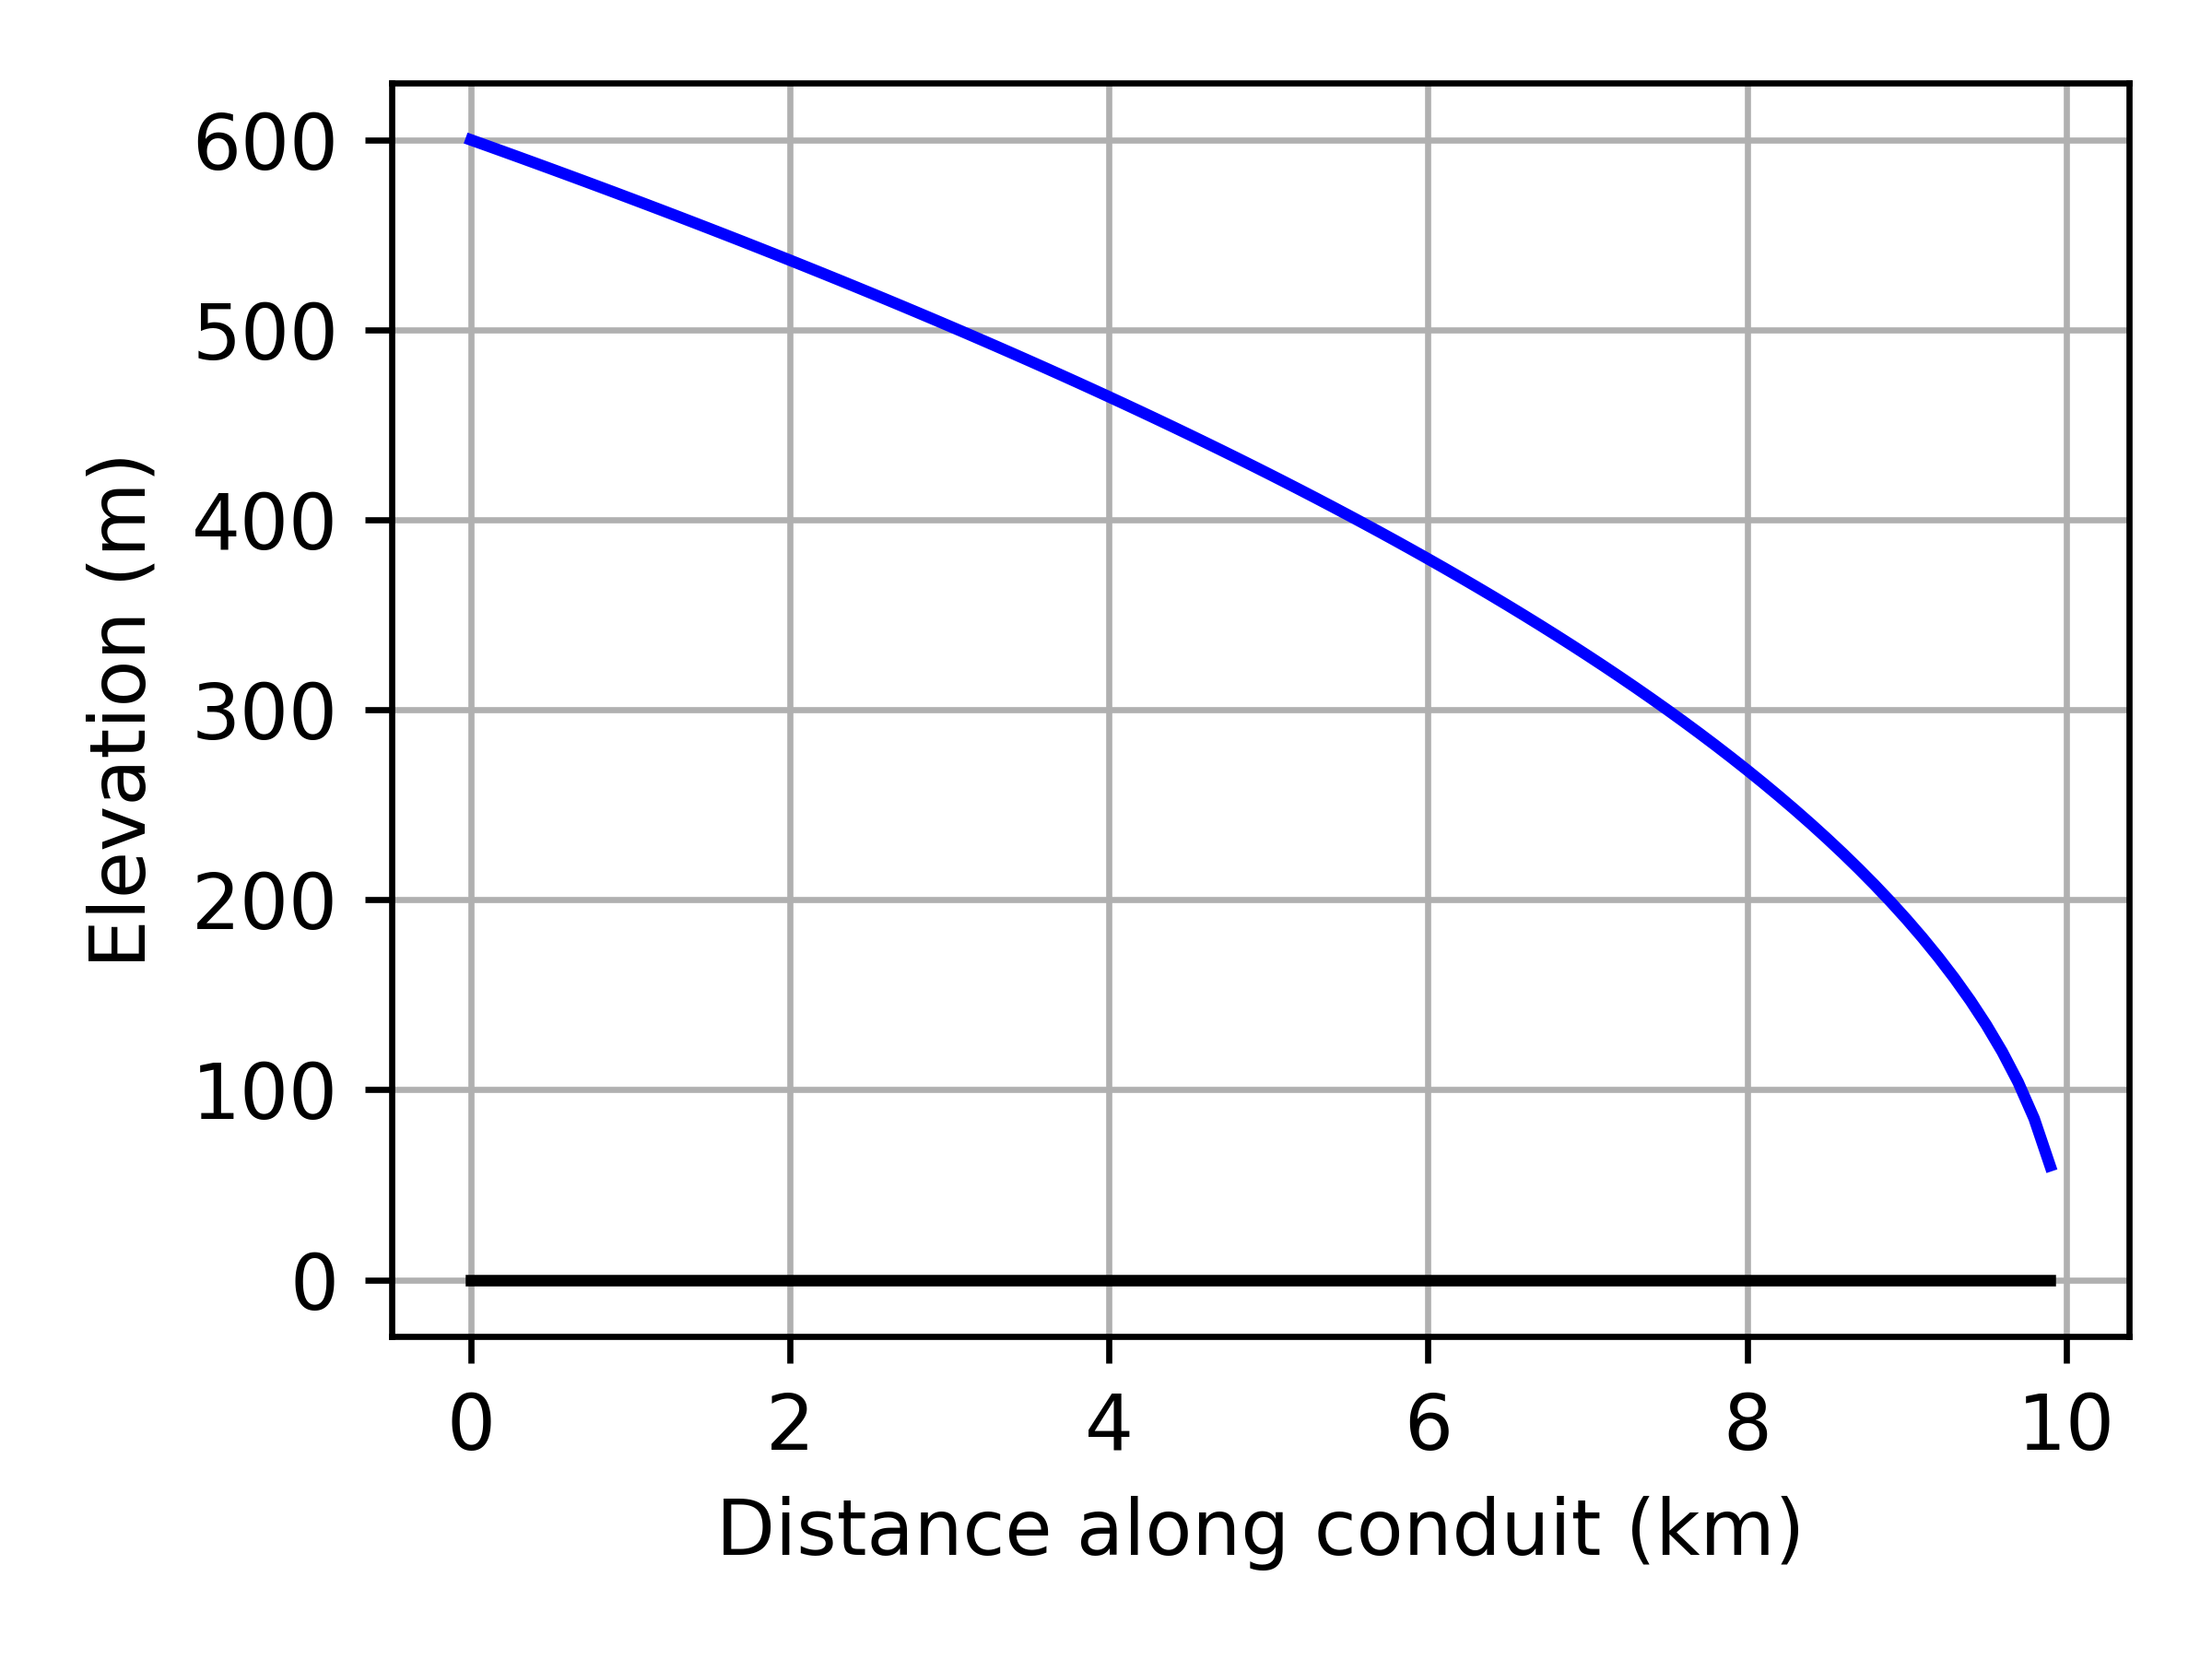
\includegraphics[width=3.5in]{domain.png}
\caption{Numerical domain for the solution of the outburst flood models. The bed is at $z_b = 0$, and the surface elevation is in blue. The surface elevation is such that $z_s(L + \Delta s) = 0$.}
\label{fig:domain}
\end{figure}

\begin{figure}[t]
\centering
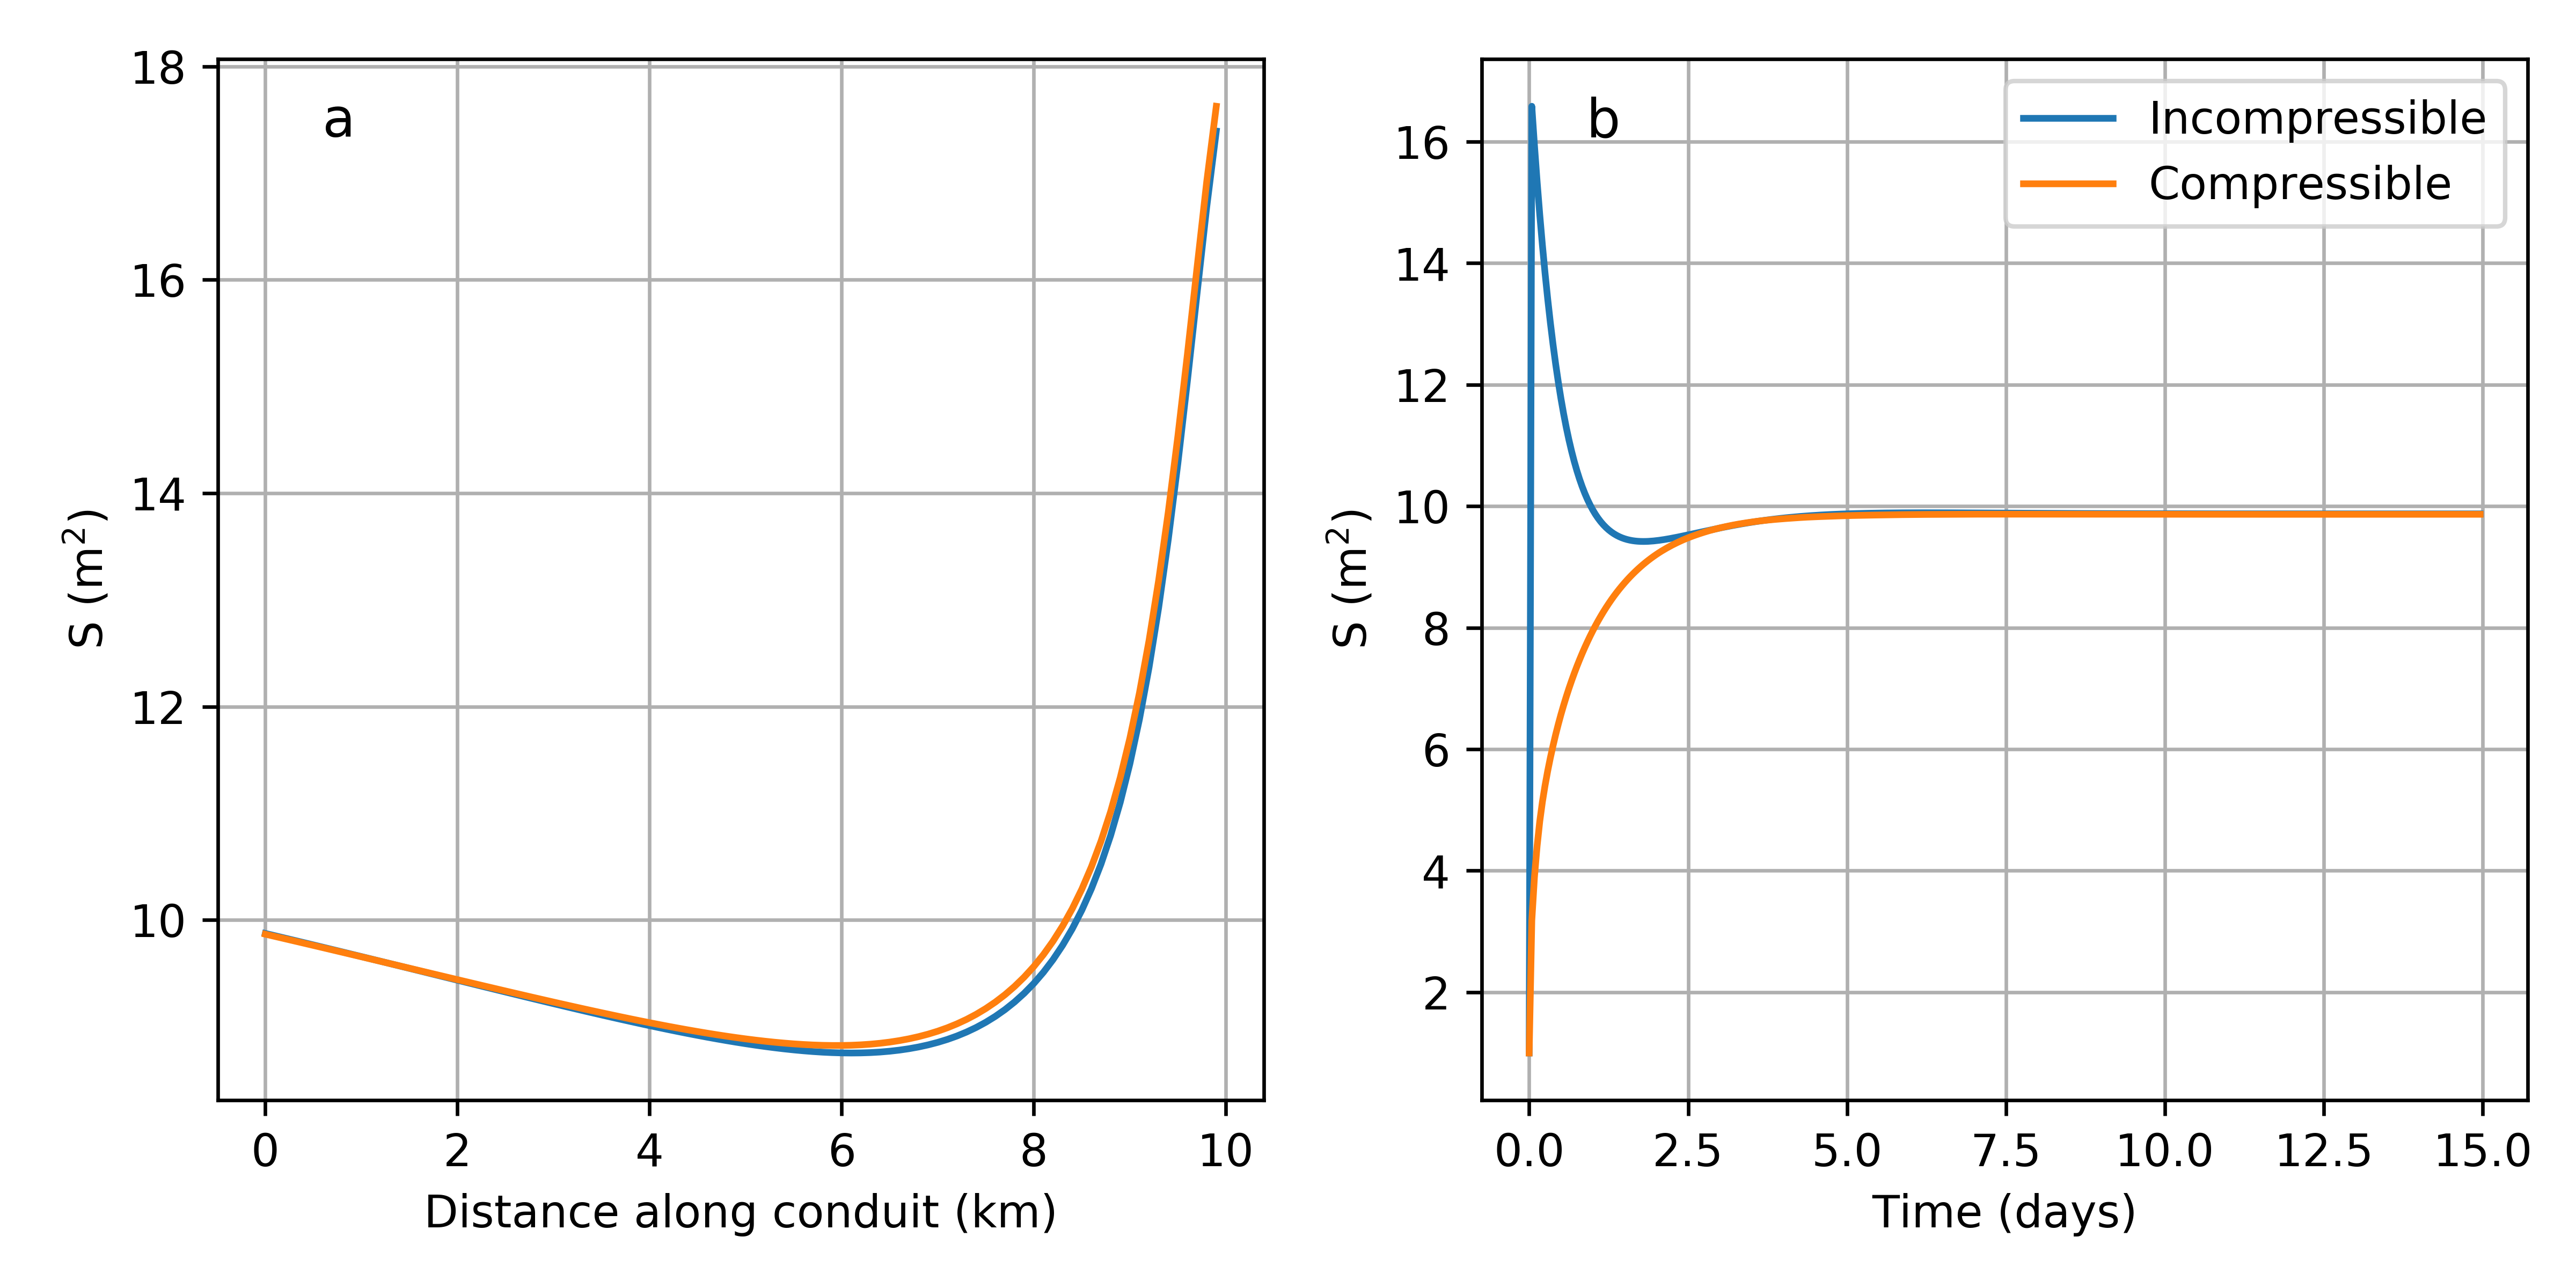
\includegraphics[width=\textwidth]{imposed_discharge_comparison.png}
\caption{Comparison of channel area at $t = \SI{30}{days}$ (a) and channel area at $s = 0$ (b) for incompressible and compressible models for the case of prescribed discharge, $Q_0 = \SI{10}{m^3.s^{-1}}$}
\label{fig:prescribed}
\end{figure}

\section{Results}
To better isolate differences between the compressible and incompressible models, we apply the conduit equations to an idealized synthetic geometry (Figure 1). Our domain has length $L = \SI{10}{km}$, with the lake outlet at $s = 0$. The bed is flat, $z_b = 0$, so that the bed slope $\frac{\partial z_b}{\partial s}$ terms vanish from the governing equations. The surface slope is a square root profile with a maximum thickness of \SI{600}{m},
\begin{linenomath*}
\begin{equation*}
z_s(s) = \frac{600}{\sqrt{L}}\sqrt{L - s}.
\end{equation*}
\end{linenomath*}
The domain is partitioned into $N = 100$ cells so that $\Delta s = \SI{100}{m}$. The incompressible model is solved with a timestep $\Delta t = \SI{3600}{s}$.

We include a small lake that drains through the subglacial conduit. The lake has an area of $500 \times 500\SI{}{m^2}$ that is uniform with depth. Initially, the water level is at the overburden pressure head level, so that $h = p_i\frac{\rho_i}{\rho_w}$.

First, we investigate the differences between the compressible and incompressible models for a prescribed lake discharge. Then, we include pressure-coupled lake discharge and explain the failure of the incompressible model. Finally, we present the full solution including pressure-coupled lake drainage with the compressible model.

\begin{figure}[tp]
\centering
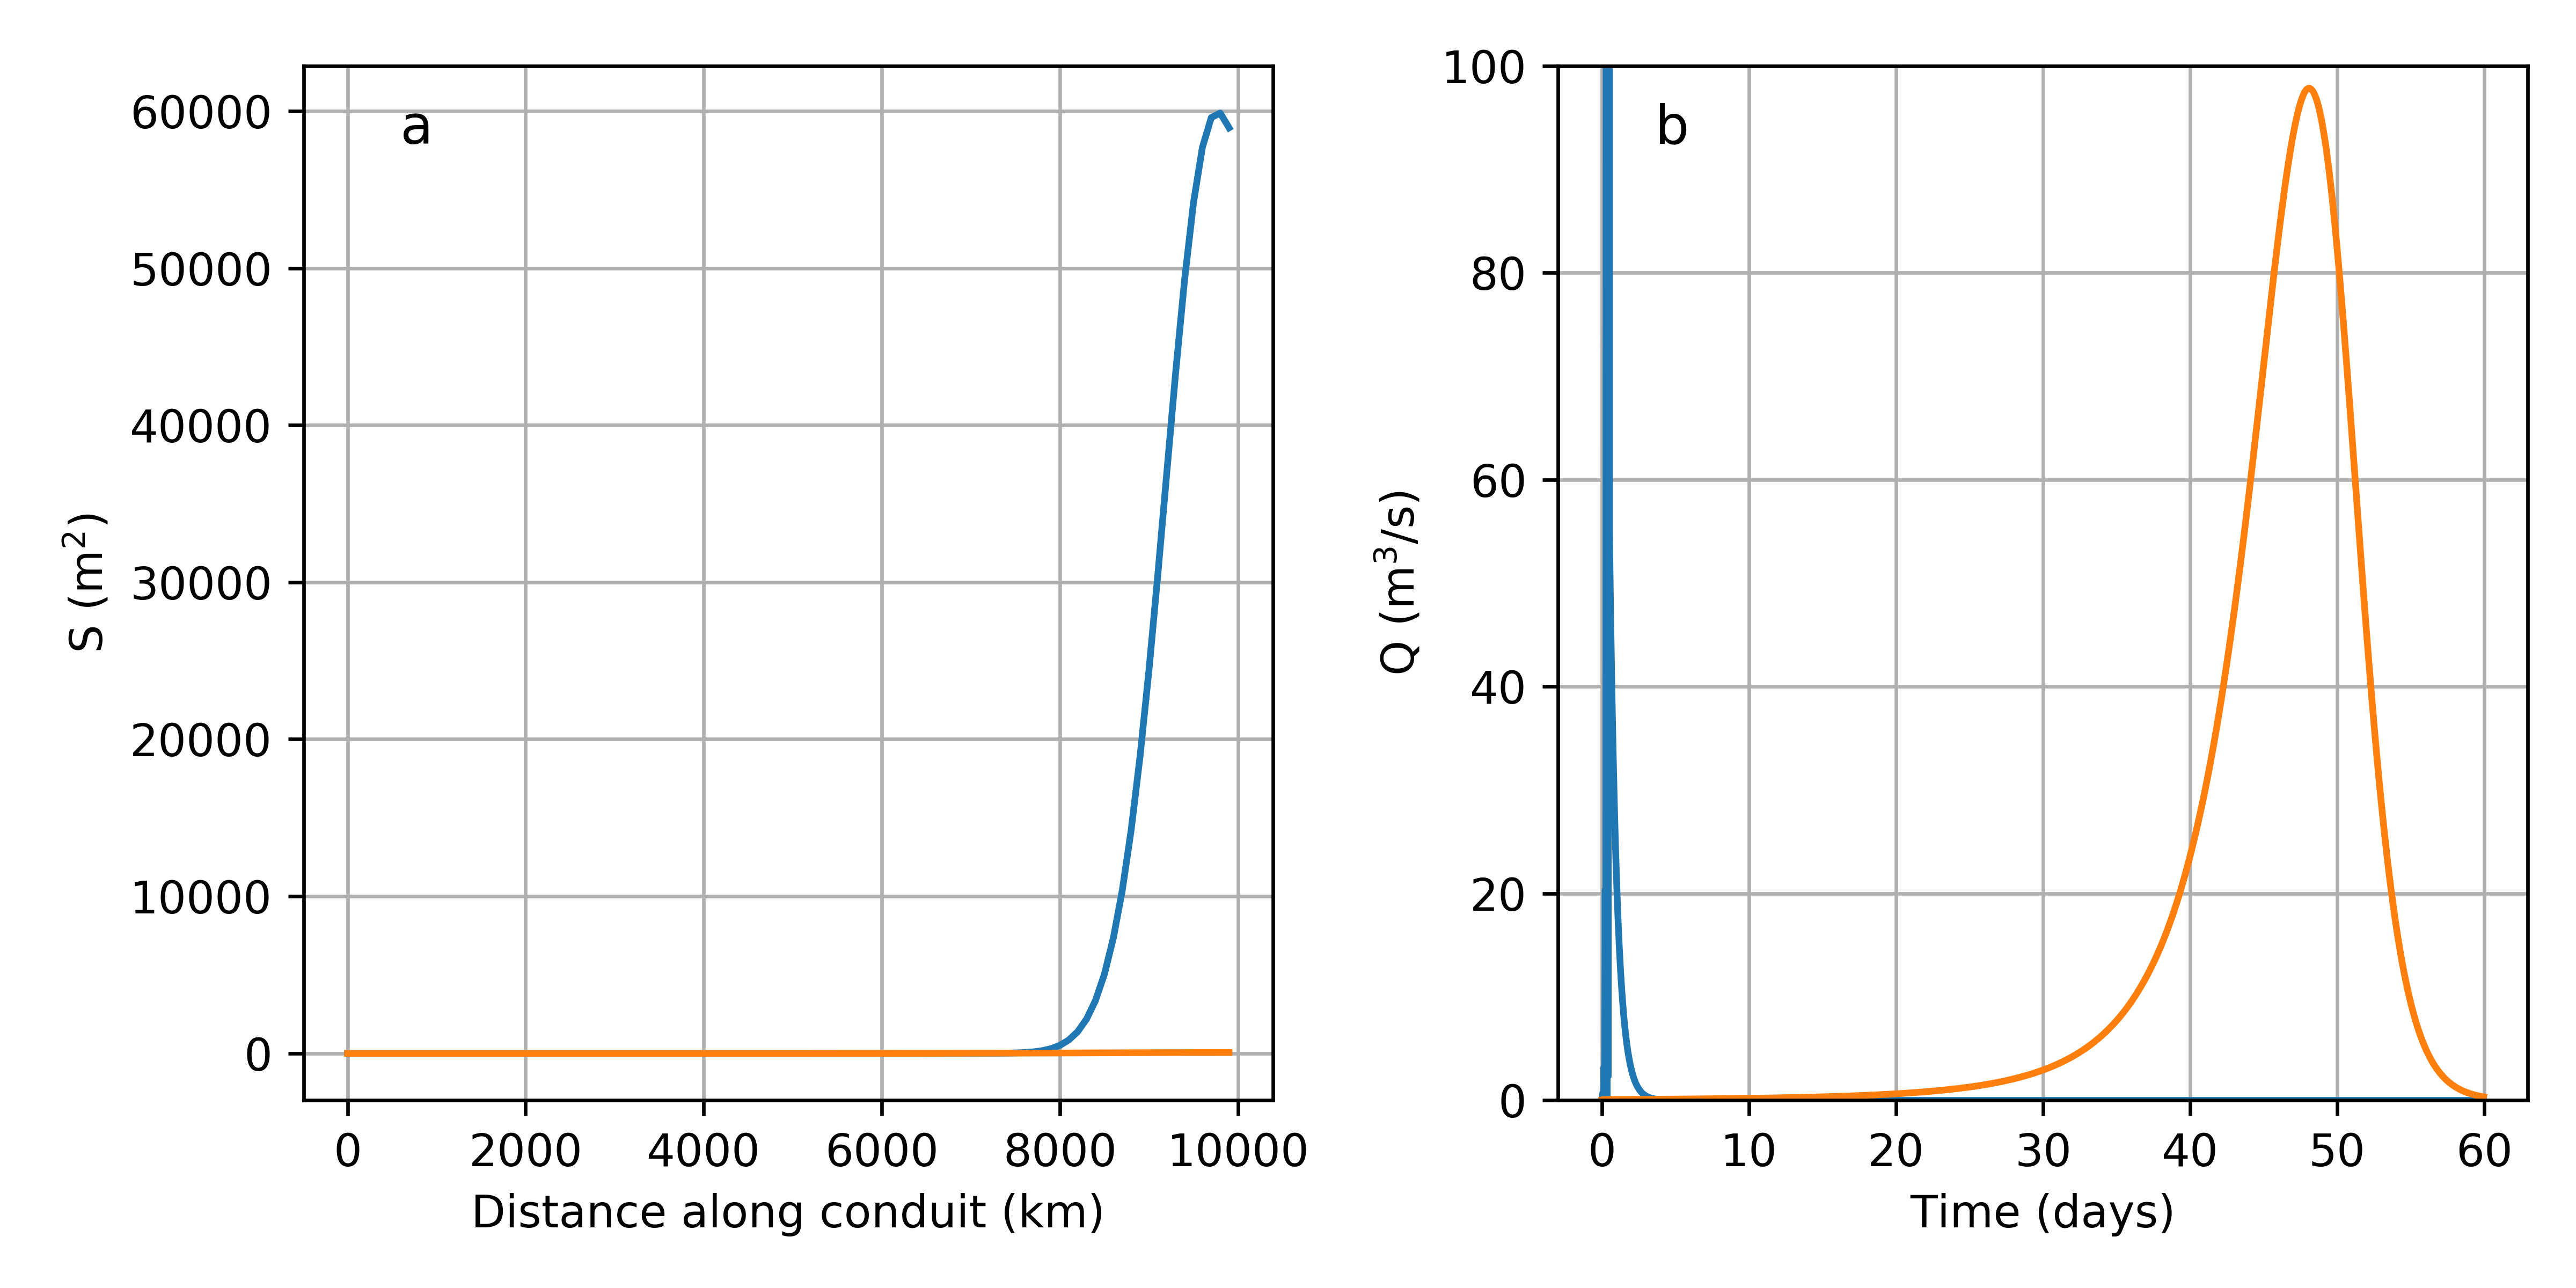
\includegraphics[width=\textwidth]{pressure_discharge_comparison.png}
\caption{Channel area at $t = \SI{60}{days}$ (a) and lake discharge timeseries (b) for incompressible and compressible models with pressure-coupled lake drainage.}
\label{fig:pressure-coupled}
\end{figure}

\subsection{Prescribed discharge: model intercomparison}
We solve the conduit equations for both incompressible ($\beta = 0$) and compressible ($\beta = \SI{1e-7}{Pa.^{-1}}$) cases for a prescribed and constant lake discharge of $Q_0 = \SI{10}{m^3.s^{-1}}$. We specify an initial uniform channel area of \SI{1}{m^2}. Since the solution for pressure and discharge is time-indpendent, we do not specify an initial condition for water pressure.

After $t = \SI{30}{days}$, the channel cross-sectional area is nearly identical between the two models (Figure \ref{fig:prescribed}). For the incompressible model, we already see some numerical issues arising from its stiffness (Figure \ref{fig:prescribed}b). Between the first and second timesteps ($\Delta t = \SI{3600}{s}$), the channel area increases by $\SI{>15}{m^2}$ due to an instantaneous increase in pressure. After $\sim\SI{3}{days}$, the incompressible solution has relaxed to match the compressible solution.


\begin{figure}[t]
\centering
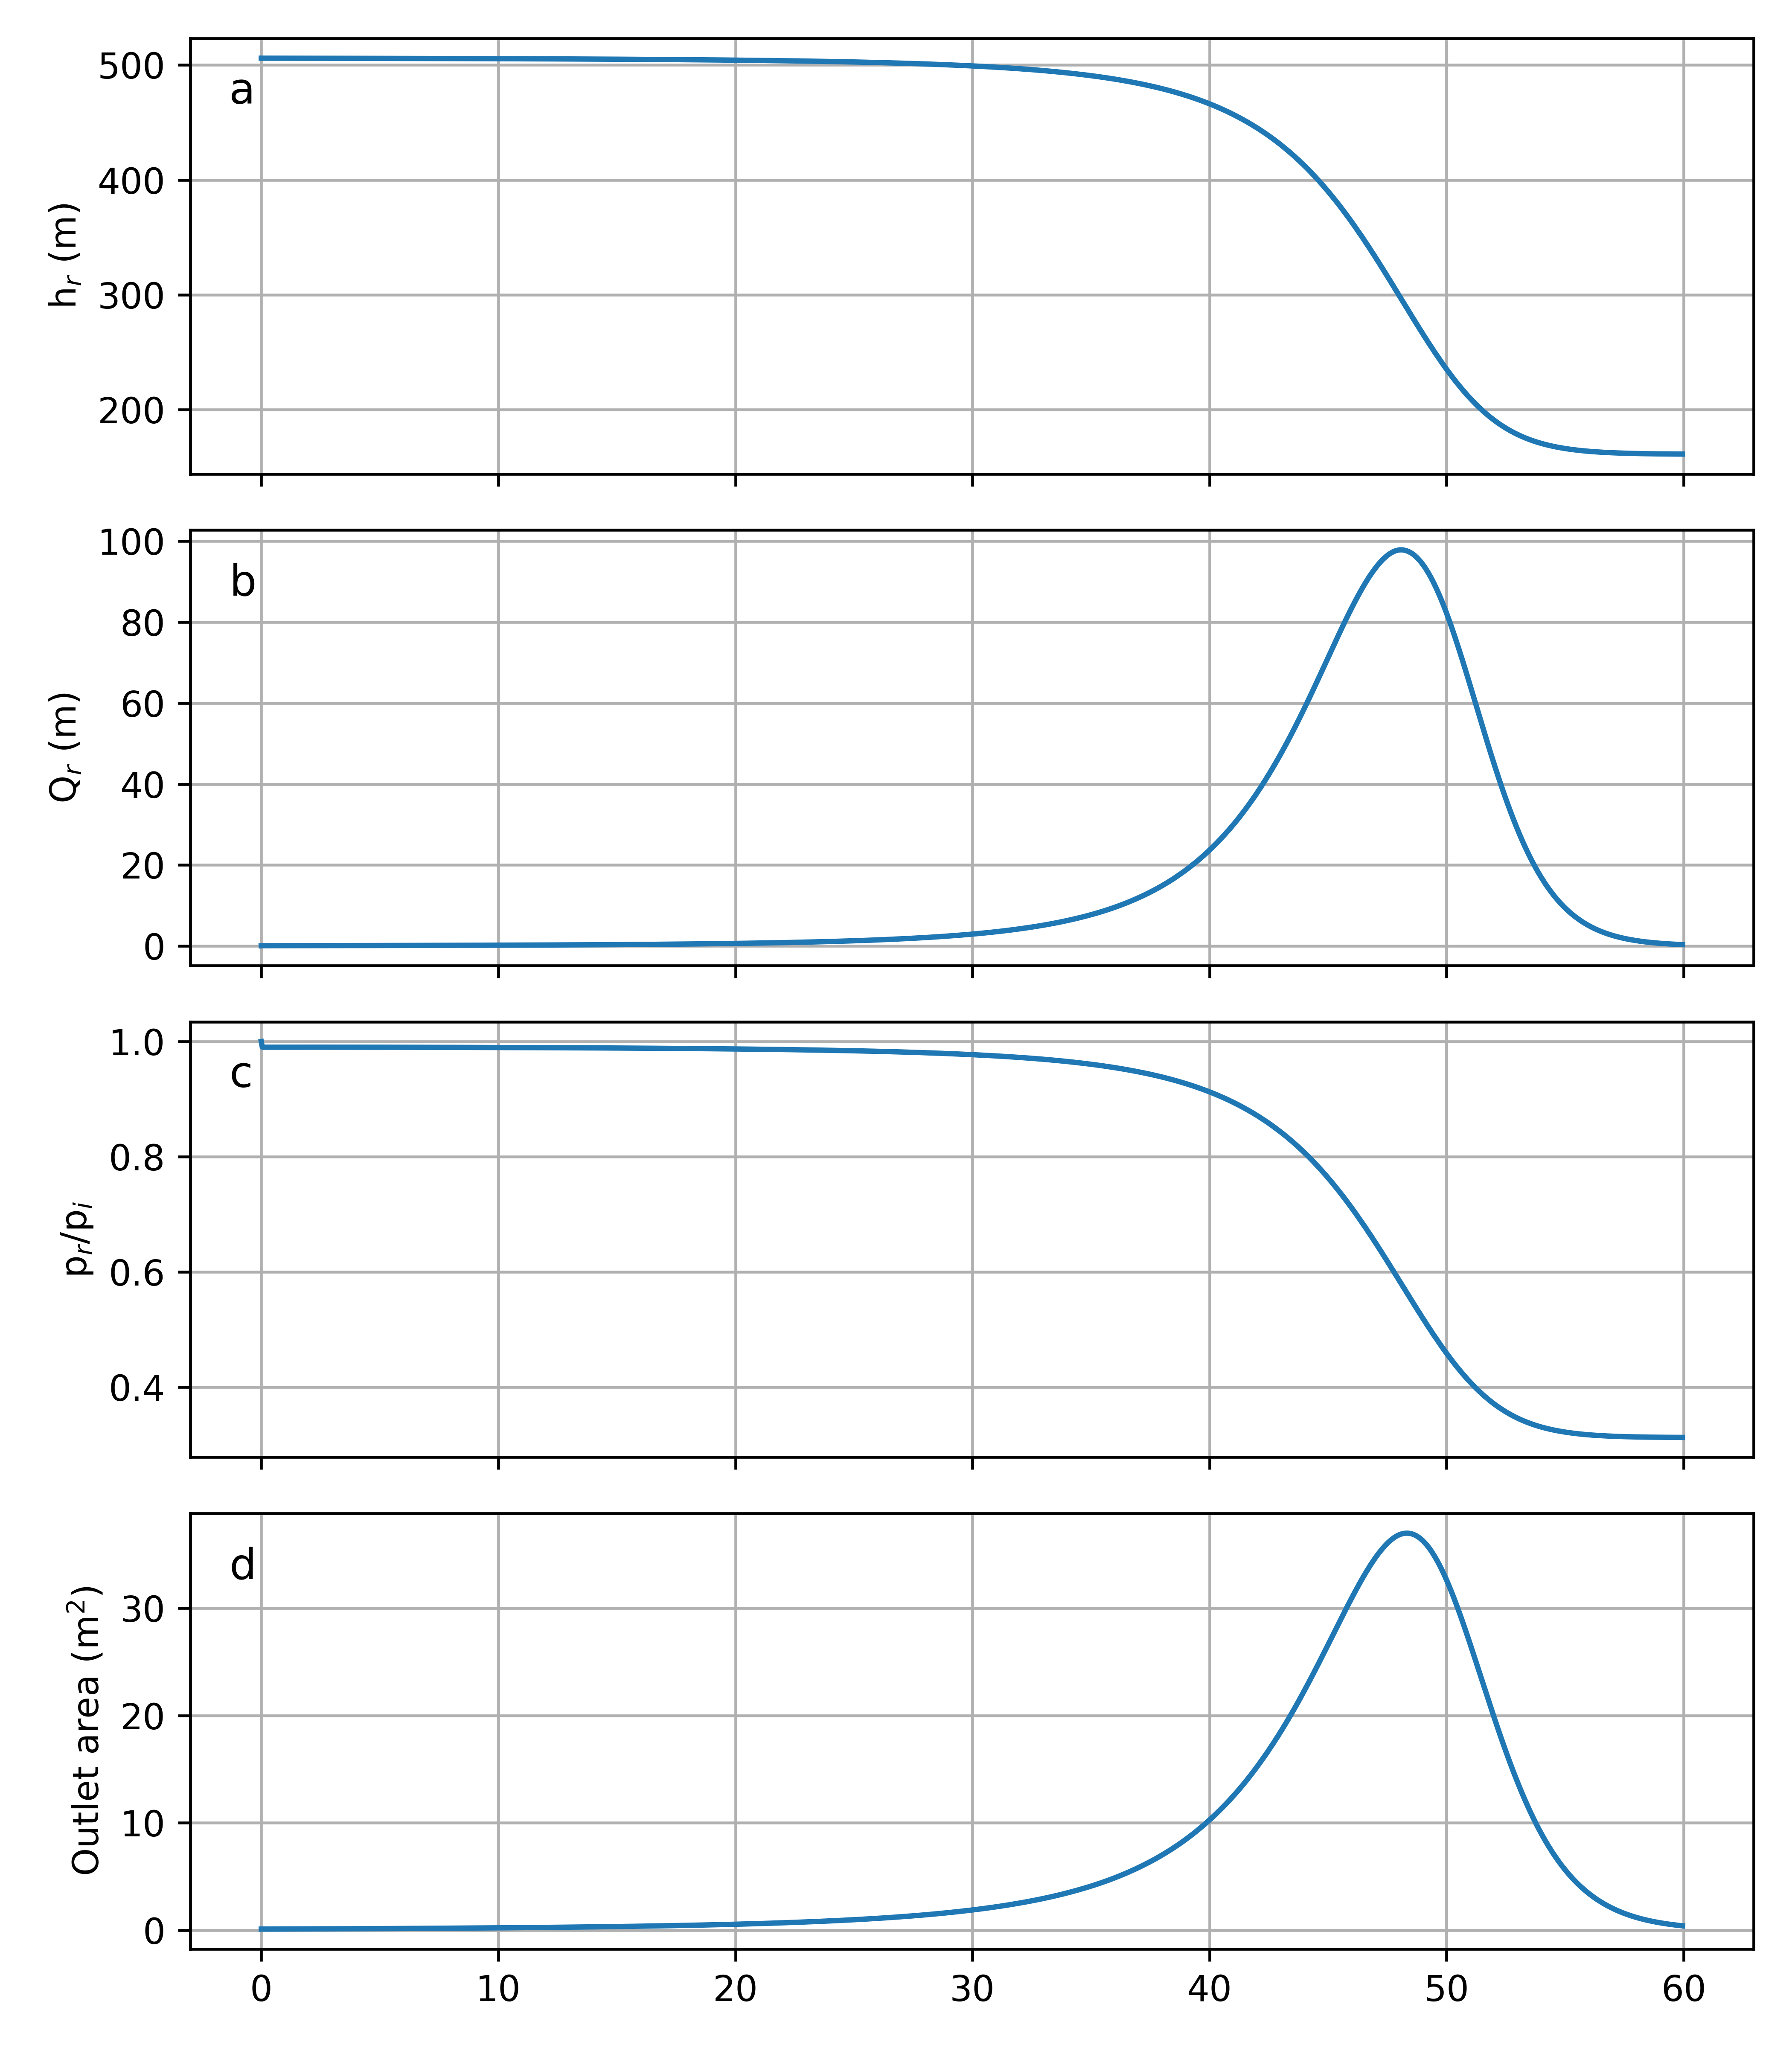
\includegraphics[width=4.5in]{compressible_pressure_drainage.png}
\caption{(a) Lake water level ($h_r$), (b) lake discharge ($Q_r$), (c) water pressure relative to ice overburden, and (d) lake outlet area for lake drainage event with $\beta = 10^{-7}\SI{}{Pa^{-1}}$.}
\label{fig:drainage-event}
\end{figure}

Note that we could easily include a more robust timestepping scheme within the incompressible model to remove the initial spike in channel area. The solutions would then agree spatially and temporally for the case of imposed lake discharge. However, a more robust solution is not pursued here due to the difficulties encountered in the next section.

\subsection{Pressure-coupled drainage}
Including pressure-coupled discharge (\ref{eq:Qreservoir}) leads to significant numerical errors for the incompressible model (Figure \ref{fig:prescribed}). At $t = 0$, instantaneous pressure fluctuations trigger rapid lake drainage, but with lake discharge oscillating between $Q = \SI{0}{m^3/s}$ and $Q > \SI{100}{m^3/s}$ between successive timesteps (Figure \ref{fig:prescribed}). The oscillation does not appear as the timestep is decreased. For the compressible model, lake discharge grows slowly for the first $\sim$30 days. The main drainage event includes rapidly increasing flow over $\sim$10 days. As explained by \citet{nye1976}, the outburst flood rapidly terminates before  the lake fully drains as creep closure increases while water pressure rapidly decreases.

Following the failure of the incompressible model, we further analyze the case of pressure-coupled lake discharge with the compressible model. We specify an initial channel area of \SI{0.1}{m^2} that is uniform along the channel length, and an initial water pressure equal to the ice overburden. 

With $\beta = 10^{-7}\SI{}{Pa^{-1}}$, the lake drainage occurs rapidly over several days approximately 50 days after the initialization (Figure \ref{fig:drainage-event}). Peak discharge is $\SI{\sim100}{m^3.s^{-1}}$, and peak channel area at the lake outlet is $\SI{\sim35}{m^2}$. The flood terminates with a lake level of $\SI{\sim 175}{m}$, and a pressure below 40\% of overburden.

\subsection{Parameter sensitivity}
In the conduit model equations (\ref{eq:consWater} -- \ref{eq:Q}), the primary unknown parameters are the friction factor $f_R$, the flow law coefficient $A$ which we have assumed to be constant, and the compressibility $\beta$. The flow-law exponent $n$ may also be viewed as an unknown, but we keep the value fixed at $n = 3$. The channel behaviour primarily depends on the ratio of frictional melt to creep closure, so that the behaviour depends on the combination of $A$ and $f_R$. For this reason, we investigate the sensitivity to $f_R$ only, holding $A$ fixed.

The parameter sensitivity is explored in Figure \ref{fig:sensitivity}. The lake discharge is highly sensitive to the friction factor but not to the compressibility for appropriate values. Decreasing the friction factor from 0.15 to 0.05 nearly doubles the peak discharge and halves the time to peak flow. For compressibility at or below $10^{-5}\SI{}{Pa^{-1}}$, discharge is insensitive to the compressibility. However, the discharge is notably suppressed and delayed for $\beta = 10^{-4}\SI{}{Pa^{-1}}$, suggesting that $\beta$ should stay below this threshold.

\begin{figure}[t]
\centering
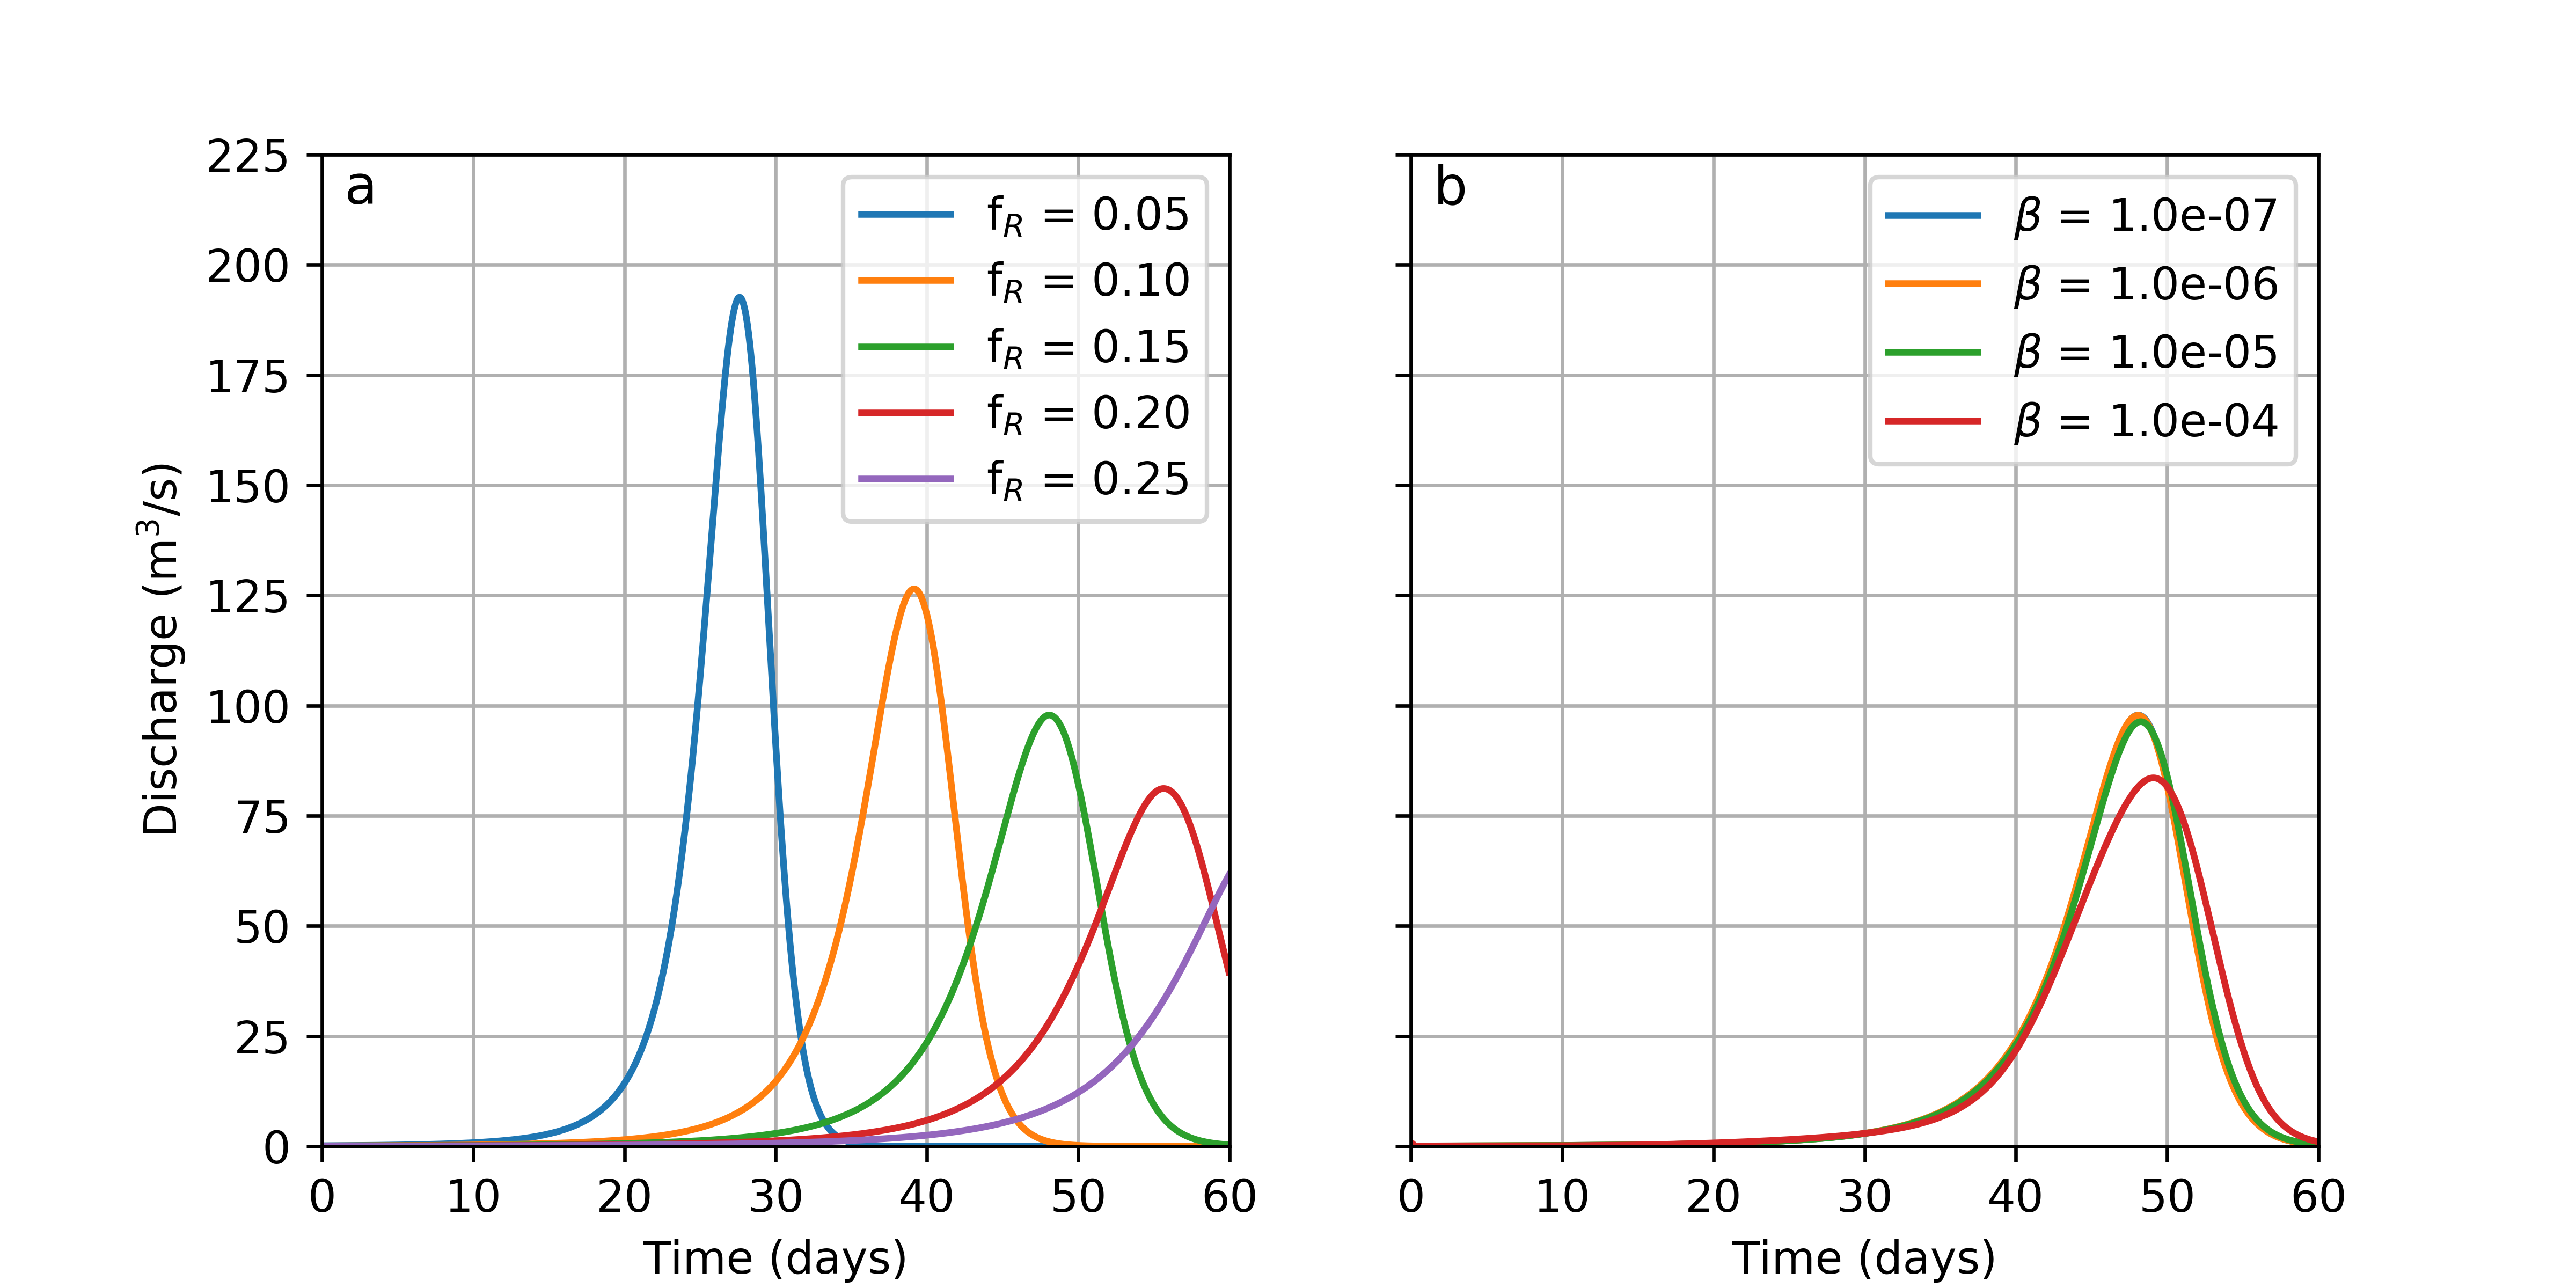
\includegraphics[width=\textwidth]{sensitivity_tests.png}
\caption{Sensitivity tests for the pressure-coupled compressible model. (a) Lake discharge sensitivity to friction factor $f_R$. (b) Sensitivity to compressibility $\beta$.}
\label{fig:sensitivity}
\end{figure}

\subsection{Sensitivity to reservoir hypsometry}
So far, we have only considered a reservoir with a constant area-depth relationship. We should expect that a realistic hypsometry, where lake area decreases with depth, will change the discharge trajectory. If lake area decreases, the lake level and therefore pressure will drop faster as the lake drains. To test the sensitivity to the reservoir hypsometry, we solve the compressible model for the same domain but with a pyramidal reservoir, such that $A_r(h) \propto h^2$, and such that the total reservoir volume is retained. With this hypsometry, the lake drainage occurs at the same time as the constant area case but with a higher peak discharge and a more rapid termination. In this case, the lake fully drains (Figure \ref{fig:hypsometry}).

\begin{figure}[t]
\centering
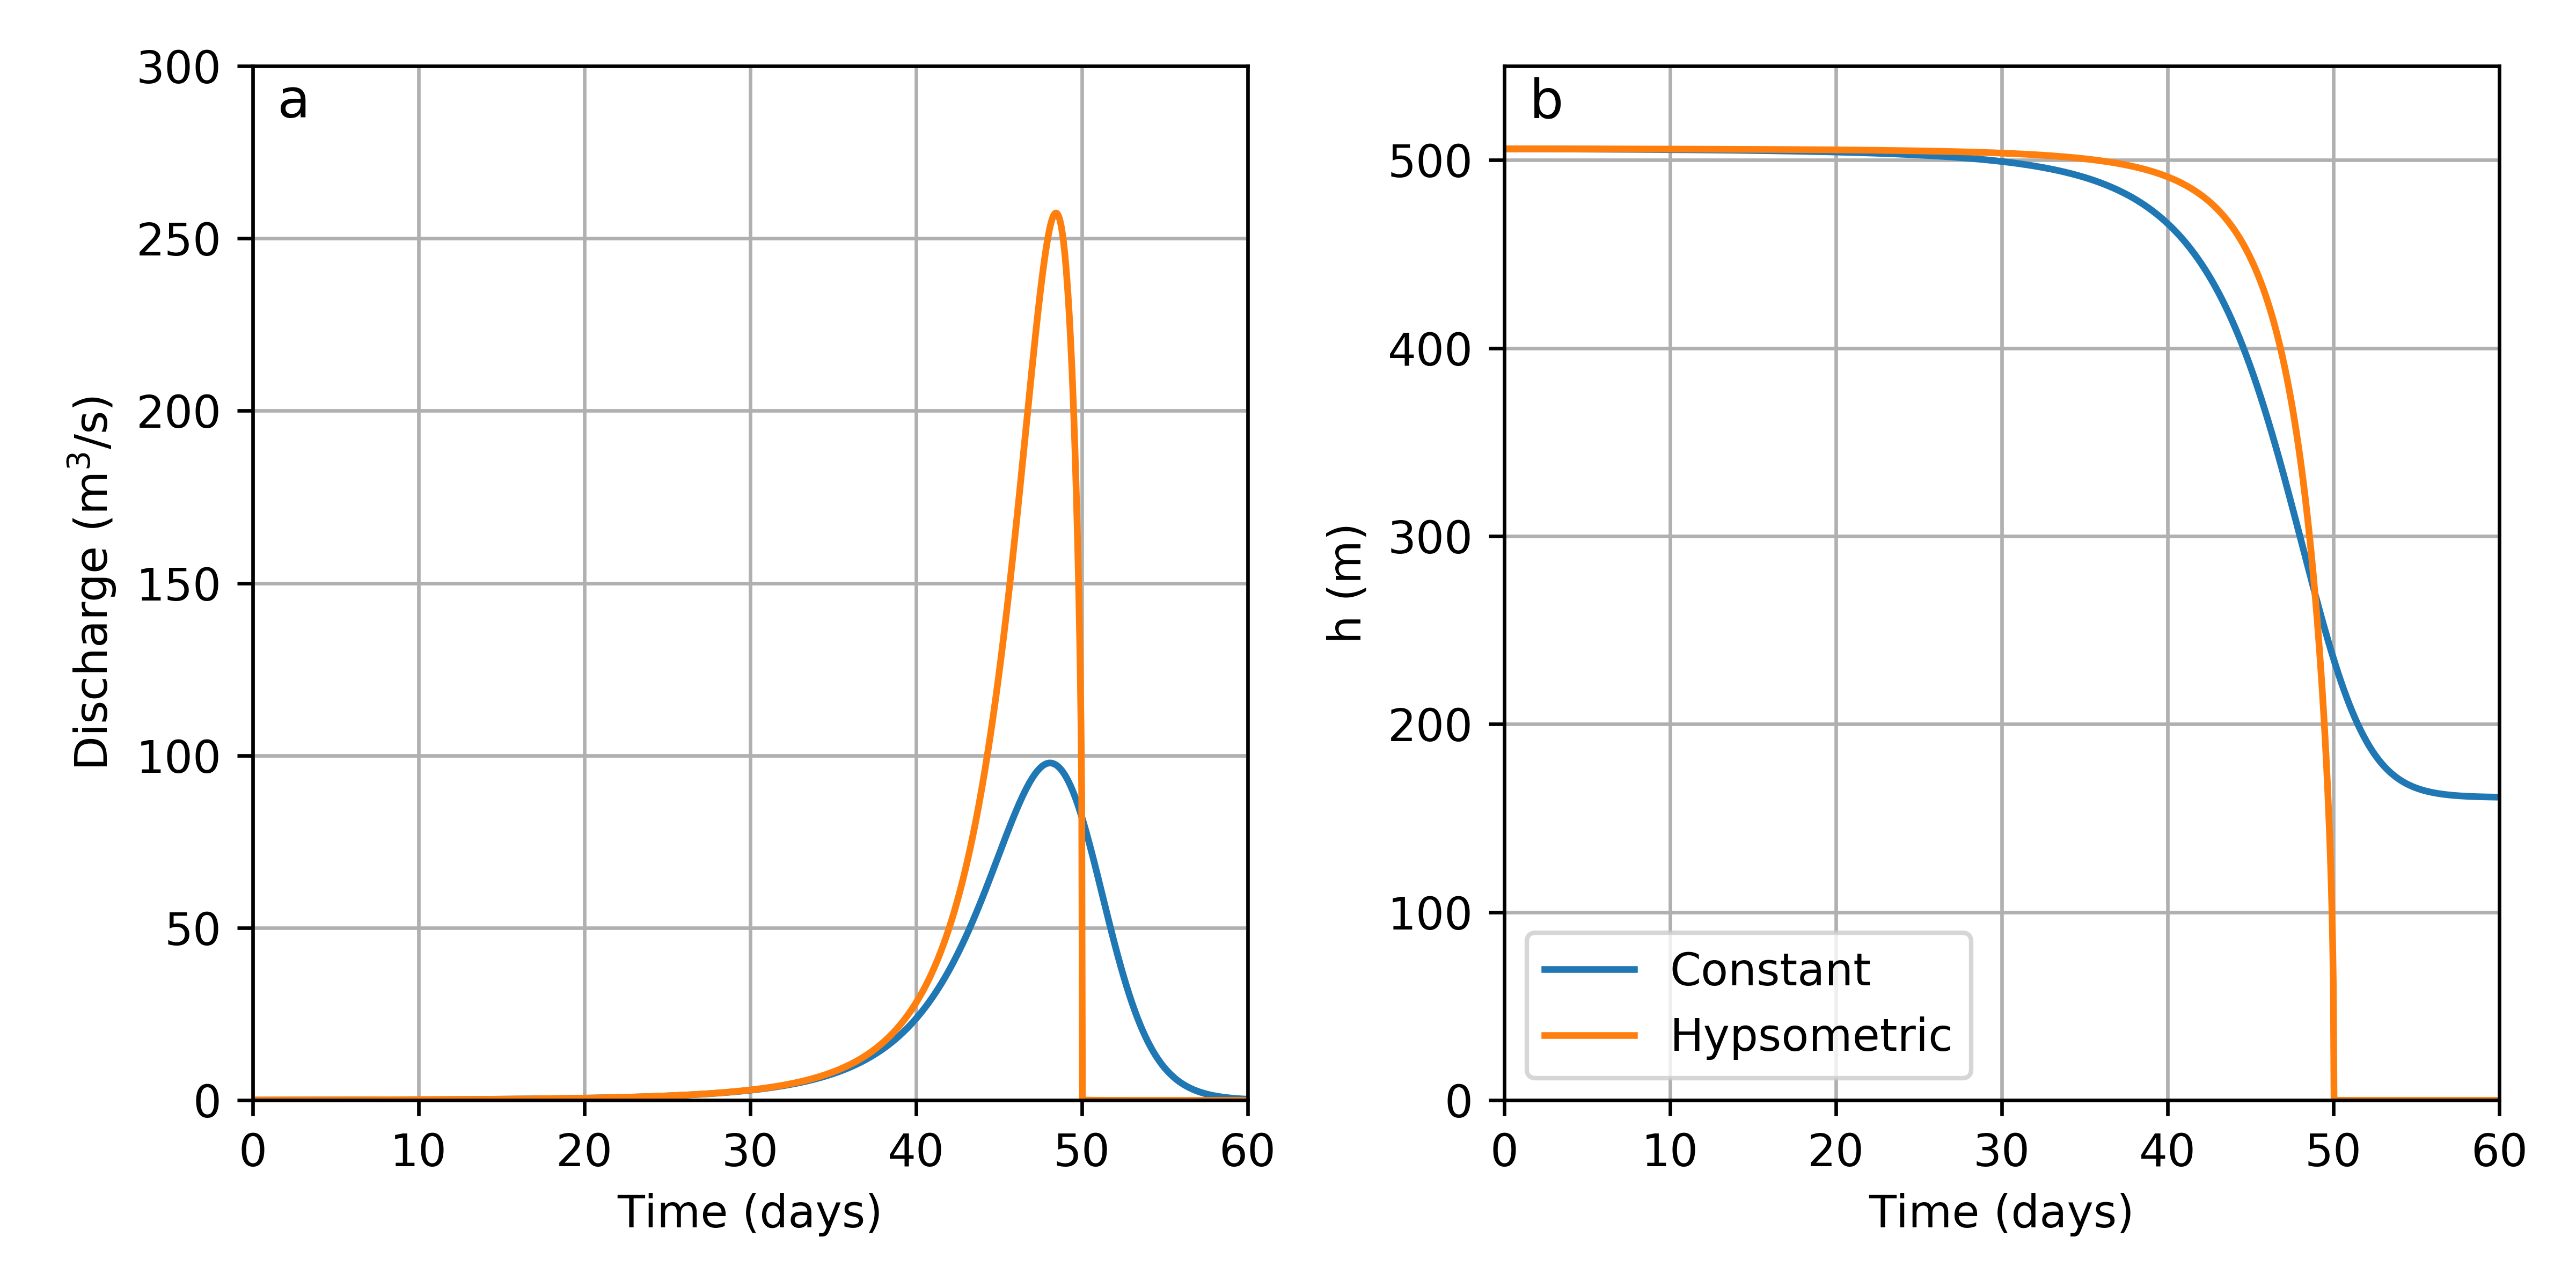
\includegraphics[width=5in]{hypsometry_discharge.png}
\caption{(a) Lake discharge and (b) lake level for a drainage event in the case of non-constant hypsometry.}
\label{fig:hypsometry}
\end{figure}


\section{Discussion}
We have presented numerical models for water flow through a subglacial conduit during a subglacial lake outburst flood. The models differ by their assumption of compressibility. The Spring-Hutter model assumes water is perfectly incompressible. The compressible model instead includes a numerical compressibility parameter $\beta$ to improve the behaviour of the numerical solution \citep{clarke2003}.

The incompressible model solves a coupled system of time-independent differential equations for water pressure and discharge. Since these equations are time-independent, pressure waves travel instantaneously. The solutions are stable in the case of prescribed lake discharge, but are prohibitively stiff due to the instantaneous propagation of pressure waves in the case of pressure-coupled lake discharge (Figure \ref{fig:pressure-coupled}). These findings align with \citet{clarke2003}, who first introduced the compressibility $\beta$ to resolve the stiffness of the model presented by \citet{spring1981}. While we have used the default value $\beta = 10^{-7}\SI{}{Pa^{-1}}$, which is higher than the physical compressibility of \SI{\sim4.5e-10}{Pa.^{-1}} \citep{clarke2003}, the solution does not differ significantly from the incompressible solution (Figure \ref{fig:prescribed}). Combined with the behaviour of the incompressible solution with pressure-coupled lake drainage (Figure \ref{fig:pressure-coupled}), we conclude that the compressible model will yield more realistic results than the incompressible model.

The pressure-coupled drainage in the case of the compressible model displays several key features noted by \citet{nye1976} and in real drainage events, for example from Grimsv\"otn \citep{flowers2004}: the majority of the discharge occurs within a short time period (several days in our model, 40 hours in the measurements shown by \citealt{flowers2004}); discharge shuts down as quickly as it ramps up; and the flood may or may not terminate before the lake fully drains. These comparisons can only be made qualitatively since we have not recreated the Grimsv\"otn geometry.

In the case of non-constant hypsometry, the lake drainage event more closely resembles the examples of \citet{clarke2003} and \citet{flowers2004}. For Hazard Lake, the flood model by \citet{clarke2003} terminates nearly instantaneously. For Summit Lake and Grimsv\"otn, the floods instead show a broader discharge peak that is qualitatively similar to ours in the case of non-constant hypsometry (Figure \ref{fig:hypsometry}). Reservoir shape is therefore important in determining the behaviour of the flood, including the peak discharge and whether the reservoir fully drains.

We have also performed parameter sensitivity tests to assess the model's sensitivity to the friction factor $f_R$ and the compressibility $\beta$ in the pressure-coupled drainage case (Figure \ref{fig:sensitivity}). Since the friction factor is difficult to directly measure, it should be possible to exploit the sensitivity to the friction factor to calibrate the friction so that the modelled flood closely matches observations. However, this sensitivity also means that using a directly measured or estimated value would be difficult, since any measurement error would result in large modelling errors.

The sensitivity to the flow law exponent $n$ has not been explored here. A higher value of $n$ should act to steepen the discharge curves in Figure \ref{fig:drainage-event}, since the creep closure will be suppressed for low effective pressures and enhanced for high effective pressures. A lower $n$ would do the opposite, resulting in a more gradual drainage event. It is possible that different exponents would change whether or not the lake drains completely in the constant hypsometry case. This sensitivity would be interesting to explore in future work.

For compressibility values up to $10^{-5}\SI{}{Pa^{-1}}$, modelled discharge is not sensitive to the compressibility (Figure \ref{fig:sensitivity}). There is very little difference in the discharge curves for $10^{-7} \leq \beta \leq 10^{-5}$, while for $\beta = 10^{-4}\SI{}{Pa^{-1}}$ the discharge curve is noticeable suppressed and delayed. We have also found little difference compared to the perfectly incompressible model (Figure \ref{fig:prescribed}) in the case of prescribed discharge. The compressibility assumption therefore seems like a good one in this application, and the value $\beta = 10^{-7}\SI{}{Pa^{-1}}$ used by \citet{clarke2003} represents a good tradeoff between numerical conditioning and discrepancy from the true value. \citet{flowers2004} instead used $\beta = \SI{1e-9}{Pa^{-1}}$, which more faithfully represents water's true compressibility. It is possible that this value is required for application to a real Grimsv\"otn outburst flood, but in our idealized case it is not necessary to use such a small value which results in slower simulations.

Beyond our simplified geometry, the flood model remains highly idealized. We have neglected a detailed treatment of heat transfer within the conduit, instead assuming that heat transfer is instantaneous. This assumption is motivated in part by simplicity, but also because models that explicitly represent heat transfer \citep[e.g.][]{clarke2003} have not been successful at recreating observed discharge temperatures \citep{flowers2004}. We have also assumed an idealized conduit with a circular cross-section. While this assumption is in line with previous work \citep{rothlisberger1972, nye1976, spring1981, spring1982, clarke2003}, it is likely that real conduits deviate from circular or semi-circular. Finally, we have assumed that conduits are fully saturated for their entire length, including the terminus region where the ice is \SI{\sim 50}{m} thick. With such thin ice it is unlikely that creep closure will be able to balance wall melt, and so we should expect some open-channel flow near the terminus. This condition could be included directly in the model by enforcing $p_w = 0$ (so that water is at atmospheric pressure) for some distance from the terminus, or by excluding regions with thin ice. However, as long as we don't draw strong conclusions from the exact channel area in this region, the saturated flow assumption should not result in large errors in the key variables, including discharge through the terminus.

\section{Conclusions}
We have presented incompressible and compressible subglacial outburst flood models and compared them in the case of synthetic, idealized geometry. The compressible model, patterned after the Spring-Hutter model \citep{spring1981, spring1982}, breaks down due to numerical stiffness in the case of pressure-coupled lake drainage. The incompressible model \citep{clarke2003, flowers2004} recreates smooth, realistic discharge hydrographs.

Since the compressible model ($\beta = 10^{-7}\SI{}{Pa^{-1}}$) aligns with the incompressible model for the case of prescribed lake discharge and is insensitive to the compressibility for $\beta < 10^{-5}\SI{}{Pa^{-1}}$, we conclude that the model does not have significant errors as a result of the compressible assumption. However, our assumption of idealized circular channel cross-section, instantaneous heat transfer, and saturated flow may result in important errors when applied to simulate real outburst floods.

Based on these idealized numerical experiments, we recommend the compressible model should be used in the realistic case where lake discharge depends on the conduit water pressure. If the compressibility value used is above the physical compressibility of water, sensitivity tests should be done to ensure the solution does not strongly depend on the compressibility. The sensitivity to the friction factor opens the possibility of statistically calibrating the model to measured outburst flood data.

The model is relatively fast and appears robust, suggesting that it can be used in interesting applications. Subglacial hydrology models \citep[e.g.][]{werder2013} already include a similar formulation coupling linked-cavity and channelized subglacial drainage. An interesting possible application is the cascading drainage of linked subglacial and ice-marginal lakes. The compressible model described here could assess whether the drainage of upstream lakes triggers or impacts the drainage of downstream lakes, and what other factors (geometric, ice dynamic) are needed to explain observed drainage patterns.

\section*{Data availability}
All code and data is available at \url{https://github.com/SFUGG/outburst_flood_model/}.

\bibliographystyle{apalike}
\bibliography{refs_A3.bib}

\clearpage
\appendix

\section{Discretization and more numerical methods}
Derivatives are approximated with finite differences. Recall that we defined the operator D in (\ref{eq:D}) as
\begin{linenomath*}
\begin{equation*}
D = \frac{\partial}{\partial s} + \frac{1}{L_f}\left(\frac{1}{\rho_i} - \frac{1}{\rho_w}\right)\left(-\rho_w g \frac{\partial z_b}{\partial s} - (1 - \gamma)\frac{\partial p_w}{\partial t}\right).
\end{equation*}
\end{linenomath*}
Numerically, we approximate the derivative operator $\frac{\partial}{\partial s}$ the operator
\begin{linenomath*}
\begin{equation}
\label{eq:Ds}
D_s^- = \frac{1}{\Delta s} \begin{bmatrix} 1 & 0 & \ldots & 0 \\ -1 & 1 & 0 \ldots \\
 & & \vdots & \\
 0 & \ldots & -1 & 1\end{bmatrix}
\end{equation}
\end{linenomath*}
As-is, this matrix operator is equivalent to a ghost cell with position $s = -\Delta s$ with value 0. Therefore, we add the imposed lake discharge $Q_0$ to the first entry of the right-hand side vector $\mathbf{y}$. 

Analogously, the upwind derivative operator is
\begin{linenomath*}
\begin{equation}
\label{eq:Dsup}
D_s^+ = \frac{1}{\Delta s} \begin{bmatrix} -1 & 1 & \ldots & 0 \\ 0 & -1 & 1 & \ldots \\ & & \vdots & \\ 0 & \ldots & 0 & -1 \end{bmatrix},
\end{equation}
\end{linenomath*}
which implicitly assumes the vector it is applied to is zero at $s = L + \Delta s$.

Now, define the vector $\mathbf{z}$ as
\begin{linenomath*}
\begin{equation}
\mathbf{z} = \frac{1}{L_f}\left(\frac{1}{\rho_i} - \frac{1}{\rho_w}\right)\left(-\rho_w g \frac{\partial z_b}{\partial s} - (1 - \gamma)D_s^+p_w \right)
\end{equation}
\end{linenomath*}
Then, the complete numerical approximation to the $D$ operator is
\begin{linenomath*}
\begin{equation}
D_{\textrm{FD}} = D_s^- + \textrm{diag}(\mathbf{z}),
\end{equation}
\end{linenomath*}
and we solve the linear system
\begin{linenomath*}
\begin{equation}
D_{\textrm{FD}}Q = \mathbf{y} + \begin{bmatrix} Q_0 \\ 0 \\ \vdots \\ 0 \end{bmatrix}.
\end{equation}
\end{linenomath*}


\end{document}
